\documentclass[11pt]{article}
\usepackage{natbib}
\usepackage{graphicx}
\usepackage{xcolor}
\usepackage[scaled]{helvet}
\usepackage[T1]{fontenc}
\usepackage[margin=0.5in]{geometry}
\usepackage[fleqn]{amsmath}
\usepackage{amssymb}
\usepackage{bm}
\usepackage{subcaption}
\usepackage{listings}
\usepackage{float}
\usepackage{tikz}
\lstset{language=Python,
    frame=single,
    breaklines=true,
    postbreak=\raisebox{0ex}[0ex][0ex]{\ensuremath{\color{red}\hookrightarrow\space}}
}

\restylefloat{figure}
\newcommand{\Prop}{\textbf{Proposition: }}
\newcommand{\Prob}{\textbf{Problem: }}
\newcommand{\Prf}{\textbf{Proof: }}
\newcommand{\Sol}{\textbf{Solution: }}
\newcommand{\grad}{\nabla}
\newcommand{\Nats}{\mathbb{N}}
\newcommand{\Ints}{\mathbb{Z}}
\newcommand{\Rats}{\mathbb{Q}}
\newcommand{\Reals}{\mathbb{R}}
\newcommand{\Comps}{\mathbb{C}}
\newcommand{\Prb}[1]{P\left( #1 \right)}
\newcommand{\PT}[1]{P\left( \text{#1} \right)}
\newcommand{\PCon}[2]{P\left( #1 \mid #2 \right)}
\newcommand{\PConT}[2]{P\left( \text{#1} \mid \text{#2} \right)}
\DeclareMathOperator{\E}{\mathbb{E}}
\DeclareMathOperator{\tr}{\textbf{tr}}
\DeclareMathOperator*{\argmin}{argmin}
\DeclareMathOperator*{\argmax}{argmax}
\newcommand{\thus}{\quad\mathlarger{\mathlarger{\mathlarger{\Rightarrow}}}\quad}
\newcommand{\wght}{\mathbf{w}}
\newcommand{\im}{\text{im }}
%%\newcommand\scalemath[2]{\scalebox{#1}{\mbox{\ensuremath{\displaystyle #2}}}}


%% Tikz stuff
\usetikzlibrary{shapes,arrows}
\usetikzlibrary{decorations.pathreplacing, decorations.pathmorphing, snakes, calligraphy}

\tikzstyle{block} = [rectangle, draw, thick, align=center, rounded corners]
\tikzstyle{boundingbox} = [very thick, gray]
\tikzstyle{dashblock} = [rectangle, draw, thick, align=center, dashed]
\tikzstyle{conc} = [ellipse, draw, thick, dashed, align=center]
\tikzstyle{netnode} = [circle, draw, very thick, inner sep=0pt, minimum size=0.5cm]
\tikzstyle{relunode} = [rectangle, draw, very thick, inner sep=0pt, minimum size=0.5cm]
\tikzstyle{line} = [draw, very thick, -latex']
\tikzstyle{arrow} = [draw, ->, thick]
\tikzstyle{mapsto} = [draw, |->, thick]

\def\checkmark{\tikz\fill[scale=0.4](0,.35) -- (.25,0) -- (1,.7) -- (.25,.15) -- cycle;}


%% Some colors stolen from ColorBrewer
\definecolor{bpurp}{HTML}{984ea3}
\definecolor{bblue}{HTML}{377eb8}
\definecolor{bgreen}{HTML}{4daf4a}
\definecolor{borange}{HTML}{ff7f00}
\definecolor{bred}{HTML}{a50f15}

% footnote without a marker
\makeatletter
\def\blfootnote{\gdef\@thefnmark{}\@footnotetext}
\makeatother



\renewcommand\familydefault{\sfdefault}
\title{A computational framework for learning and transforming task representations}
\author{Andrew Kyle Lampinen}
\date{}
\begin{document}
\maketitle

Humans exhibit substantial cognitive flexibility. We can use our knowledge of a task to adapt to novel variations on our first try. For example, imagine you are playing poker with your friends, and one of them says ``next round, let's try to lose.'' You will be able to perform well, despite the new goal directly contradicting your prior goal. Alternatively, suppose your friend says ``next round, threes will be jokers.'' You will be able to play this variation, even if you have never played it before. For an example from another domain, imagine your friend shows you a blue car, and then tells you that their car looks similar, except that it is red. You will be able to combine these pieces of knowledge to recognize their car, despite never having seen it before. Humans can adapt our knowledge to a new situation on our first try. 

By contrast, while deep learning models can achieve human (or super-human) accuracy at games \citep{Silver2017,Vinyals2019} and object recognition \citep{Szegedy2016}, they are unable to flexibly adapt their knowledge of these tasks \citep{Lake2016}. How could a deep learning model trained to win at poker reuse that knowledge to try to lose? How could a model trained to recognize one car adapt to recognize that car in a different color? Many deep learning models cannot, even in principle.  

Observations like these have formed a key piece of contemporary critiques of deep learning models as cognitive models \citep{Lake2016,Marcus2018}. These critiques echo criticisms of the generalization capabilities of neural networks from the earlier days of connectionism \citep{Fodor1988}. Can deep learning serve as a cognitive model, or does it lack some of the ingredients of human intelligence, as these critiques suggest? 

In this dissertation, I bring new light to this debate, by proposing and demonstrating a novel approach to adaptation in deep learning models. The method is based on interpreting the types of adaptation above as transformations of tasks. For example, there might be a ``try-to-lose'' transformation that would transform poker to a losing variation of poker, chess to a losing variation of chess, etc. I therefore propose a general framework for both learning task representations, and learning to transform those task representations in order to adapt to new tasks. This allows deep learning models to adapt to new tasks before they have experienced them, based on the relationship between the new tasks and prior tasks. That is, it allows deep learning models to flexibly reuse their knowledge of a task to adapt to novel variations of that task. In fact, the approach demonstrates 80-90\% performance on novel tasks across a broad range of domains, including simple card games and video games, and visual classification. Furthermore, this adaptation allows the model to learn the novel tasks much more efficiently.  

This work therefore has broad implications. It addresses fundamental questions about the computational approaches necessary for flexible intelligence, and how that flexibility can contribute to later learning. This has implications for cognitive science, neuroscience, and philosophy of mind. In addition, I demonstrate the approach within several important contemporary artificial intelligence paradigms, including visual classification and deep reinforcement learning. It may therefore also be of interest to artificial intelligence and machine learning researchers who wish to build more flexible artificial intelligence.

\section{The method: adaptation as task transformation}

My approach is based on the idea that many tasks can be seen as mappings from inputs to outputs. For example, poker can be seen as a mapping of hands to bets (Fig. \ref{fig:HoMM:tasks_as_mappings:basic}), and visual classification can be seen as a mapping from images to classifications.  


\section{Selected experimental results}

\section{Conclusions}

\bibliographystyle{apalike}
\bibliography{arrr}

\begin{figure}[H]
\centering
\begin{subfigure}{0.33\textwidth}
\centering
\begin{tikzpicture}[auto]
%% a) basic task
\draw[boundingbox, draw=gray, fill=white] (-2.25, -2.5) rectangle (2.25, 2.5);
\node[gray, text width=2cm, align=center] at (0, 2.1) {Poker task};
\begin{scope}[shift={(0,-0.5)}]
\node[text width=0.5cm] at (-1, -1.3) {\includegraphics[width=0.5cm]{2-HoMM/figures/4_of_hearts.png}};
\node[text width=0.5cm] at (-0.85, -1.25) (pokerin0) {\includegraphics[width=0.5cm]{2-HoMM/figures/2_of_spades.png}};
\node[text width=0.5cm] at (0.85, -1.25) (pokerout0) {\bf ?};
\path[mapsto] (pokerin0) to (pokerout0);
\end{scope}
\begin{scope}[shift={(0,0.5)}]
\node[text width=0.5cm] at (-1, -1.3) {\includegraphics[width=0.5cm]{2-HoMM/figures/3_of_spades.png}};
\node[text width=0.5cm] at (-0.85, -1.25) (pokerin0) {\includegraphics[width=0.5cm]{2-HoMM/figures/4_of_hearts.png}};
\node[text width=0.5cm] at (0.85, -1.25) (pokerout0) {\bf \$1};
\path[mapsto] (pokerin0) to (pokerout0);
\end{scope}
\begin{scope}[shift={(0,1.5)}]
\node[text width=0.5cm] at (-1, -1.3) {\includegraphics[width=0.5cm]{2-HoMM/figures/ace_of_spades.png}};
\node[text width=0.5cm] at (-0.85, -1.25) (pokerin0) {\includegraphics[width=0.5cm]{2-HoMM/figures/2_of_spades.png}};
\node[text width=0.5cm] at (0.85, -1.25) (pokerout0) {\bf \$2};
\path[mapsto] (pokerin0) to (pokerout0);
\end{scope}
\begin{scope}[shift={(0,2.5)}]
\node[text width=0.5cm] at (-1, -1.3) {\includegraphics[width=0.5cm]{2-HoMM/figures/4_of_hearts.png}};
\node[text width=0.5cm] at (-0.85, -1.25) (pokerin0) {\includegraphics[width=0.5cm]{2-HoMM/figures/ace_of_spades.png}};
\node[text width=0.5cm] at (0.85, -1.25) (pokerout0) {\bf \$0};
\path[mapsto] (pokerin0) to (pokerout0);
\end{scope}

\end{tikzpicture}
\caption{A basic task.} \label{fig:HoMM:tasks_as_mappings:basic}
\end{subfigure}
\begin{subfigure}{0.33\textwidth}
\centering
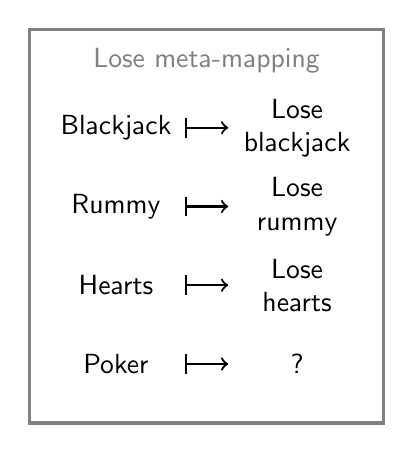
\begin{tikzpicture}[auto]
\draw[boundingbox, draw=gray, fill=white] (-2.25, -2.5) rectangle (2.25, 2.5);

\node[gray, align=center] at (0, 2.1) {Lose meta-mapping};
\begin{scope}[shift={(0,-0.5)}]
\node[text width=1.5cm, align=center] at (-1.15, -1.25) (metain0) {Poker};
\node[text width=1.5cm, align=center] at (1.15, -1.25) (metaout0) {?};
\path[mapsto] (metain0) to (metaout0);
\end{scope}

\begin{scope}[shift={(0,0.5)}]
\node[text width=1.5cm, align=center] at (-1.15, -1.25) (metain0) {Hearts};
\node[text width=1.5cm, align=center] at (1.15, -1.25) (metaout0) {Lose hearts};
\path[mapsto] (metain0) to (metaout0);
\end{scope}

\begin{scope}[shift={(0,1.5)}]
\node[text width=1.5cm, align=center] at (-1.15, -1.25) (metain0) {Rummy};
\node[text width=1.5cm, align=center] at (1.15, -1.25) (metaout0) {Lose rummy};
\path[mapsto] (metain0) to (metaout0);
\end{scope}

\begin{scope}[shift={(0,2.5)}]
\node[text width=1.5cm, align=center] at (-1.15, -1.25) (metain0) {Blackjack};
\node[text width=1.5cm, align=center] at (1.15, -1.25) (metaout0) {Lose blackjack};
\path[mapsto] (metain0) to (metaout0);
\end{scope}
\end{tikzpicture}
\caption{A task transformation.} \label{fig:HoMM:tasks_as_mappings:meta}
\end{subfigure}
\caption[Basic tasks and meta-mappings.]{Basic tasks and task transformations. (\subref{fig:HoMM:tasks_as_mappings:basic}) Basic tasks can be seen as mappings from inputs to outputs, for example, from poker hands to bets. (\subref{fig:HoMM:tasks_as_mappings:meta}) Task transformations are higher-order tasks, which take a basic task as input, and output a transformed version of that task, for example, switching from winning to losing a game.} \label{fig:HoMM:tasks_as_mappings}
\end{figure}

\end{document}
